% Wash U. McKelvey Engineering thesis template

% Use one of the following:
%\documentclass[mastersthesis,12pt]{wuthesis}
\documentclass[phdthesis,12pt]{wuthesis}

%%%%%%%%%%%%%%%%%%%%%%%%%%%%%%%%%%%%%%%%%%%%
% Enter the information requested in the following fields to ensure it is used everywhere that is needed in the front matter of the thesis.
%%%%%%%%%%%%%%%%%%%%%%%%%%%%%%%%%%%%%%%%%%%%

%% Enter your name as it should appear on the thesis
\renewcommand{\thesisauthorfirstname}{Ima}
\renewcommand{\thesisauthorlastname}{Graduatin}

%% Enter your previous degrees, if any
%\renewcommand{\thesisauthorpreviousdegrees}{, J.D.}

%% Enter department/program name (must be formatted exactly as shown in appendix of McKelvey thesis guidelines)
\renewcommand{\thesisdepartment}{Department of Computer Science \& Engineering}

%% Enter hthe name of your degree; if uncertain, consult your supervisor or program director.
\renewcommand{\thesisfield}{Computer Science}

%% Enter month and year of graduation (MUST be one of May, August, or December, reflecting the end of the semester in which your degree will be conferred). DO NOT use the month in which you will actually defend or submit the thesis document if earlier than the above.
\renewcommand{\thesismonth}{May}
\renewcommand{\thesisyear}{2023}

%% Enter title of thesis
\renewcommand{\thesistitle}{Template for Formatting of McKelvey Master's Theses and Doctoral Dissertations}

%% Enter the copyright holder ONLY if different from \thesisauthor above 
%\renewcommand{\thesiscopyrightholder}{\thesisauthor}

%% Enter name of your committee chair (generally the same as your supervisor)
\renewcommand{\thesischair}{Alan Turing}

%% list all your committee members *other* than the chair in alphabetical order by last name
\renewcommand{\thesiscommittee}{
    Ralph Alpher \\
    Hans Bethe \\
    George Gamow \\
    Grace Hopper \\
    Richard Tapia}

%%%%%%%%%%%%%%%%%%%%%%%%%%%%%%%%%%%%%%%%%%%%%%%%%%%%%%%%%%%%%%%%%%

% Include any LaTeX packages you want to use here with \usepackage. Also add any preamble declarations that you want to apply to the entire thesis.

% Suggested package to support inclusion of images
\usepackage{graphicx}

% Suggested settings for formatting URLs and hypertext references
\usepackage{xcolor}
\usepackage{hyperref}
\hypersetup{
    colorlinks,
    linkcolor={red!50!black},
    citecolor={blue!50!black},
    urlcolor={blue!80!black}
}

%%%%%%%%%%%%%%%%%%%%%%%%%%%%%%%%%%%%%%%%%%%%%%%%%%%%%%%%%%%%%%%%%%
%%
%% Include a separate LaTeX file for each chapter of the thesis immediately after the \mainmatter tag below.
%%
%% Front-matter text (acknowledgements, abstract, optional dedication, optional preface) are specified inthesis-front.tex.
%%
%%%%%%%%%%%%%%%%%%%%%%%%%%%%%%%%%%%%%%%%%%%%%%%%%%%%%%%%%%%%%%%%%%

\begin{document}

\frontmatter
%
%  Front matter for thesis or dissertation
%
% The user should 
%  * uncomment the lines to add a list of abbreviations if desired
%  * provide text for the required Acknowledgments section and Abstract section below.
%  * uncomment the Dedication section if desired and provide a dedication.

% NOTE: do not put any text in the thesistitlepage or thesiscopyrightpage sections. To create the content for these pages, change the appropriate fields in thesis-main.tex. This will ensure that the contents of these pages are positioned and formatted correctly. 

%% Generate the title page.
\thesistitlepage
      
%% Generate the copyright page.
\thesiscopyrightpage

\begin{singlespace}
\setcounter{page}{2}
\tableofcontents

\cleardoublepage
\phantomsection
\addcontentsline{toc}{chapter}{\listfigurename}
\listoffigures

\cleardoublepage
\phantomsection
\addcontentsline{toc}{chapter}{\listtablename}
\listoftables

%% If you want a list of abbreviations, uncomment the following lines and create a file abbrvs.tex with \nomenclature entries for all your abbreviations and notation. See the nomencl package documentation for details on how to create and format the entries in the list.
%\cleardoublepage
%\phantomsection
%\makenomenclature
%\input{abbrvs}
%\printnomenclature

\end{singlespace}

% Acknowledgment section is REQUIRED.
\begin{thesisacknowledgments}
Use the \emph{required} acknowledgments section to thank people who have helped you complete your thesis, either professionally (e.g., colleagues and advisors) or personally (family and friends).  If your work was supported by a fellowship or a grant to your advisor, you should also acknowledge that support here, in a form something like the following:

This work was supported by NSF award ABC-1234567.
\end{thesisacknowledgments}

%% Uncomment next section and provide text to generate an optional dedication page.
%\begin{thesisdedicationpage}  
%To my parents.
%\end{thesisdedicationpage}

\cleardoublepage
\phantomsection

% Abstract section is REQUIRED.
%
% Previously, the Library's guidance was that this abstract should be limited to 350 words to fit within limits imposed by various abstract collection services. It's not clear if this limit still exists.
\begin{thesisabstract}
The thesis abstract gives a brief overview of your work. The abstract will be indexed by various bibliographic services, so make sure that it is likely to rank highly in searches related to your work. It's likely that many more people will read your abstract, as a search result, than will read the actual thesis. Historically, there was a strict limit of 350 words for dissertation abstracts, which was imposed by the bibliographic services. It's not clear if this limit still exists, but it is probably longer than you actually want for your abstract.  This abstract has been padded out to about 250 words.

Lorem ipsum dolor sit amet, consectetur adipiscing elit. Cras ultrices porta ante ac scelerisque. Phasellus orci nisl, blandit semper congue et, pulvinar et metus. Suspendisse at congue lorem. Vestibulum sodales id felis a ultricies. Cras nec vulputate lectus. Donec condimentum lacinia sapien vitae molestie. Fusce dignissim finibus lectus, eu accumsan neque porttitor vel. Suspendisse a lobortis nisi, et rhoncus tellus. Curabitur eget fringilla nisi. Vestibulum finibus ligula nisl, in cursus augue fermentum nec. Quisque posuere nulla feugiat velit aliquet, lobortis finibus arcu pulvinar. Vivamus id pellentesque nulla. Curabitur interdum mollis luctus. Ut dapibus tortor quis faucibus imperdiet.

Proin vulputate diam ligula, vestibulum posuere erat scelerisque nec. Fusce lobortis nisl ac est pretium, sit amet eleifend massa tempor. Nam aliquet eu libero eget fermentum. Aliquam sit amet sodales diam. In et urna sapien. Donec venenatis aliquet ante non vestibulum. Cras iaculis eu nibh ut congue. Nulla quis. 

\end{thesisabstract}

% If adding a preface to the main thesis, uncomment the next two lines and provide the body of the preface in the included file. The chapter heading must be the word "Preface".
%\chapter{Preface}
%\input{preface}

\mainmatter
\chapter{How To Use the Template}
\label{cpt1}

This is the McKelvey School of Engineering LaTeX template for doctoral dissertations and master's theses. Using this template will help you produce a document compliant with the School's formatting guidelines.

Not every detail of the formatting guidelines can be encapsulated in a LaTeX template. For a narrative description of the guidelines, please see the School's Microsoft Word thesis template, which can be found as part of our \href{https://engineering.wustl.edu/offices-services/student-services/graduate-student-services/thesis-dissertation-submission.html}{thesis and dissertation submission procedures}. But you should be confident that using this LaTeX template will produce a document that complies with the School's requirements for spacing, margins, indentation, page numbering, chapter and section titles, and front matter formatting. Moreover, LaTeX's Computer Modern font family, which is the default for this template, is accepted as an alternative to the Times family specified in the Word template.

To use this template, you will need to review and edit two files: the top-level document (\texttt{thesis-main.tex}) and the front-matter file (\texttt{thesis-front.tex}).  You need not and \emph{should not} modify the class file \texttt{wuthesis.cls} at all.

\section{Top-Level Document}

The file \texttt{thesis-main.tex} is the top-level document for your thesis. At the top of this file, select the appropriate document type (master's thesis or doctoral dissertation) and then edit the fields that follow to provide the title, author, committee, and other information that will appear on the title page and in the abstract.  Note that the department/program name must be written exactly as described in the appendix of the Word template.

After filling in the fields at the top of the file, specify any LaTeX packages and configuration settings that should apply to the thesis document. You should then include the actual thesis chapters as shown using LaTeX's \texttt{\textbackslash include} command.  If your thesis has a preface, uncomment the two preface lines and provide the preface as a separate \texttt{.tex} file. If your thesis has appendices, include these after the \texttt{\textbackslash appendix} line at the bottom of the file to ensure that they will be correctly numbered and formatted.

Finally, \texttt{thesis-main.tex} creates the bibliography for your document~\cite{Lovecraft1928} using BibTeX. If desired, you can change the bibliography style to whatever is appropriate for your discipline. Reference information may be added to the provided \texttt{.bib} file.

\section{Front Matter}

The file \texttt{thesis-front.tex} creates the front-matter sections of the thesis.  Much of the front matter is generated automatically from the fields you provide in \texttt{thesis-main.tex}, but there are a few sections that require you to provide your own text.  They are:

\begin{itemize}

\item List of Abbreviations (\textit{optional}) -- uncomment the indicated lines in the front-matter file and provide a \texttt{.tex} file listing all your abbreviations and notation. This template uses the LaTeX \texttt{nomencl} package, which formats the list for you; see that package's documentation for details.

\item Acknowledgments (\textbf{required}) -- write the text of your acknowledgments page in the provided \texttt{\textbackslash thesisacknowledgments} environment.

\item Abstract (\textbf{required}) -- write the text of your abstract in the provided \texttt{\textbackslash thesisabstract} environment.

\item Dedication (\textit{optional}) -- if you wish to produce a dedication page separate from your acknowledgments, uncomment the \texttt{\textbackslash thesisdedicationpage} environment and write a brief dedication.

\end{itemize}
\emph{You should not add to or modify the contents of the front-matter document}, other than filling in the items listed above.

\section{Advice on Figures and Tables}

When including a figure or table in your thesis, remember that the caption will be copied verbatim into the List Figures or List of Tables in the front matter.  This means that you will potentially end up with a paragraph for each entry in those lists, which looks odd.

% Note: use the bracketed version of caption, i.e. \caption[short-version]{text} to produce a separate, shortened version of the caption for the LoF or LoT.

\begin{figure}
    \centering
    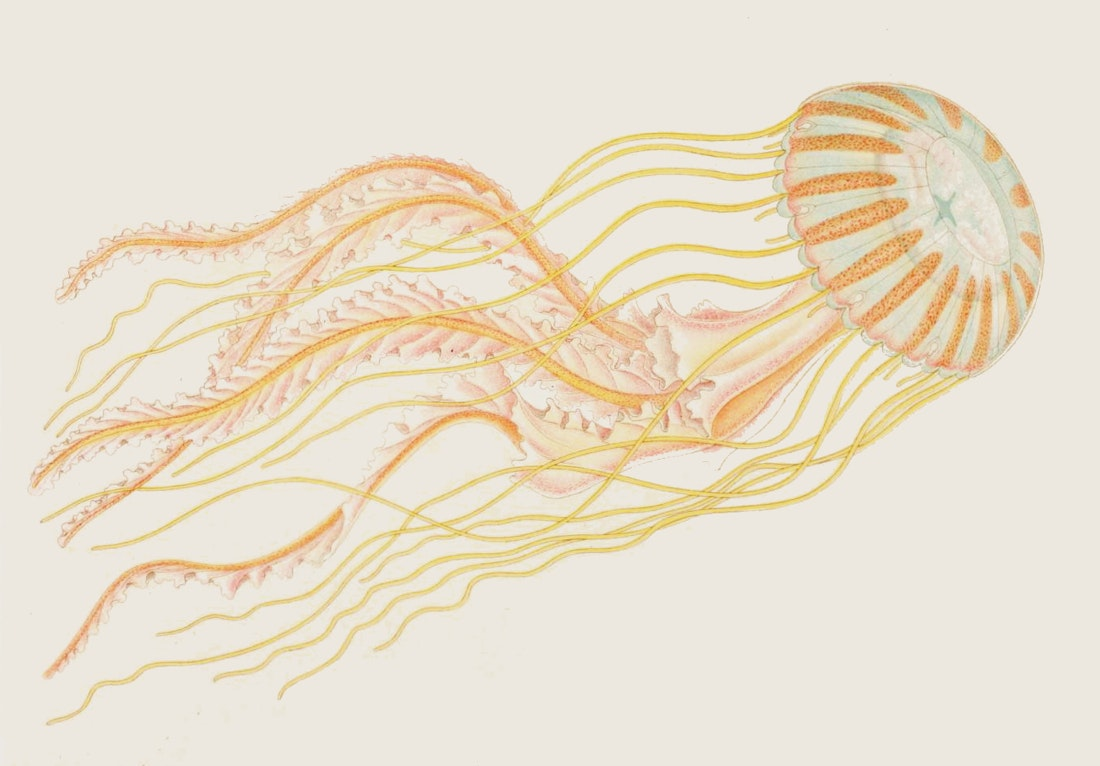
\includegraphics[width=0.6 \textwidth] {jellyfish}
    \caption[A Picture of a Jellyfish]{Jellyfish, from A.~G. Meyer, \textit{Medusae of the World}, 1910. It is venomous and squishy.}
    \label{fig:jelly}
\end{figure}

You can supply a \emph{short caption} for a figure or table that replaces the full caption in the front matter.  To do this, include the short caption in square brackets after the \texttt{\textbackslash caption} command and before the regular caption, as shown in the LaTeX source for Figure~\ref{fig:jelly} and Table~\ref{tab:fish}.

\begin{table}[b]
\centering
    \caption[A Table of Fish]{Number and color of assorted fish.  Here, fishy fishy fish!}
    \label{tab:fish}
    \begin{tabular}{|c|c|}
    \hline
         One Fish & Two Fish  \\
         Red Fish & Blue Fish \\
    \hline
    \end{tabular}
\end{table}


%\include{thesis-chapter2}
%\include{thesis-chapter3}
%\include{thesis-chapter4}
%\include{thesis-chapter5}

% Generate the bibliography.
\bibliographystyle{abbrv}
\begin{spacing}{1.0}
\bibliography{thesis-references}
\end{spacing}

% Uncomment the next line if you want to force every reference in the .bib file to appear in the final document, whether or not it was \cite'd.
%\nocite{*}

% Uncomment next lines to generate appendices, if desired.
\appendix
\chapter{Syllogisms}

My saucepans are the only things I have that are made of tin. \\
I find all your presents very useful. \\
None of my saucepans are of the slightest use. \\

No potatoes of mine, that are new, have been boiled. \\
All my potatoes in this dish are fit to eat. \\
No unboiled potatoes of mine are fit to eat. \\

No one takes in the Times, unless he is well educated. \\
No hedgehogs can read. \\
Those who cannot read are not well educated.

(\textit{Source: Lewis Carroll})
%\include{thesis-appendixB}

\end{document}
